\chapter{Position, Speed, and Acceleration}

Let's say that you get in a car and drive 45 km/hour for two hours in
one direction. Your position will be $2 \times 45 = 90$ km from where
you started. We could plot your velocity and your position during those two hours:

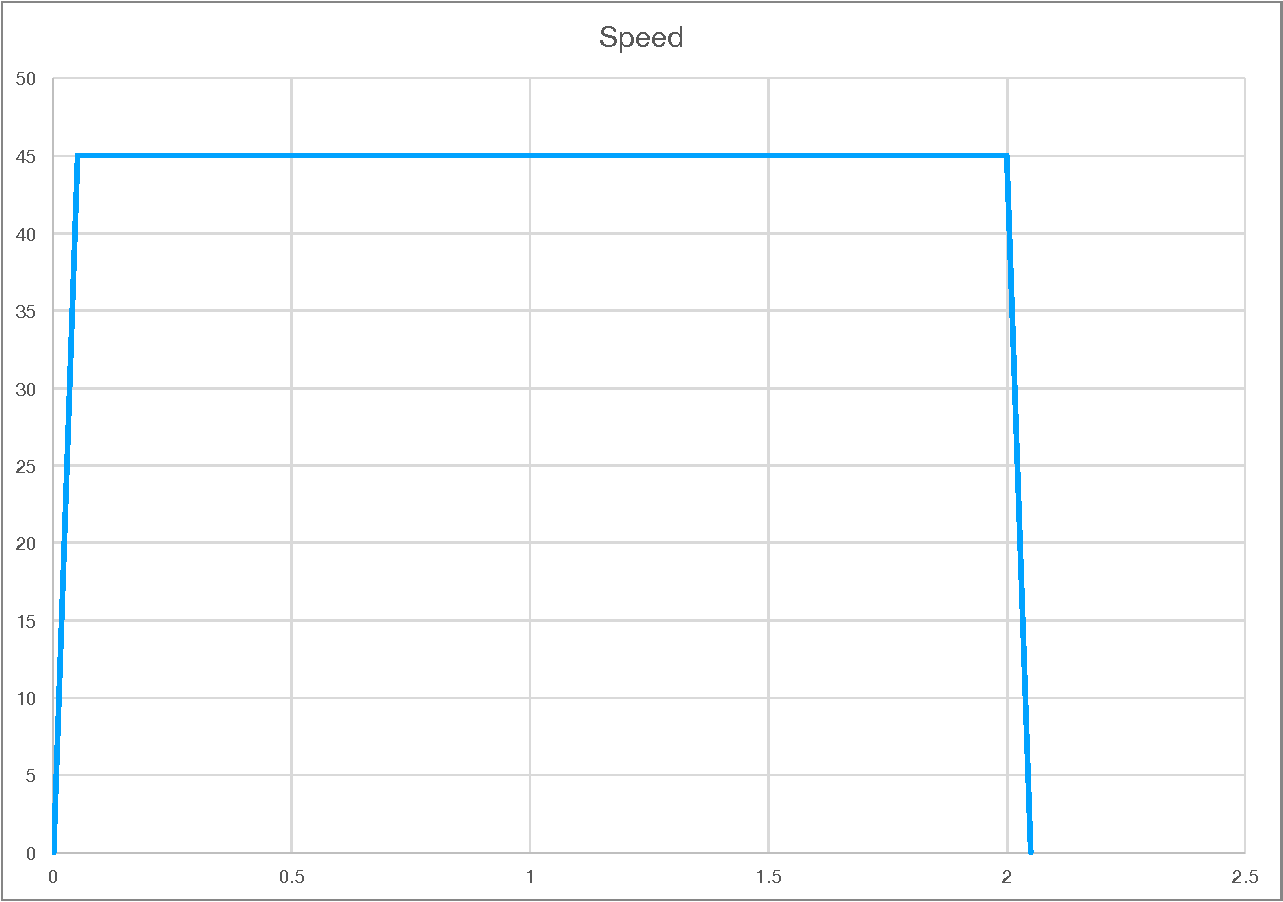
\includegraphics[width=0.7\textwidth]{speed_simple.pdf}

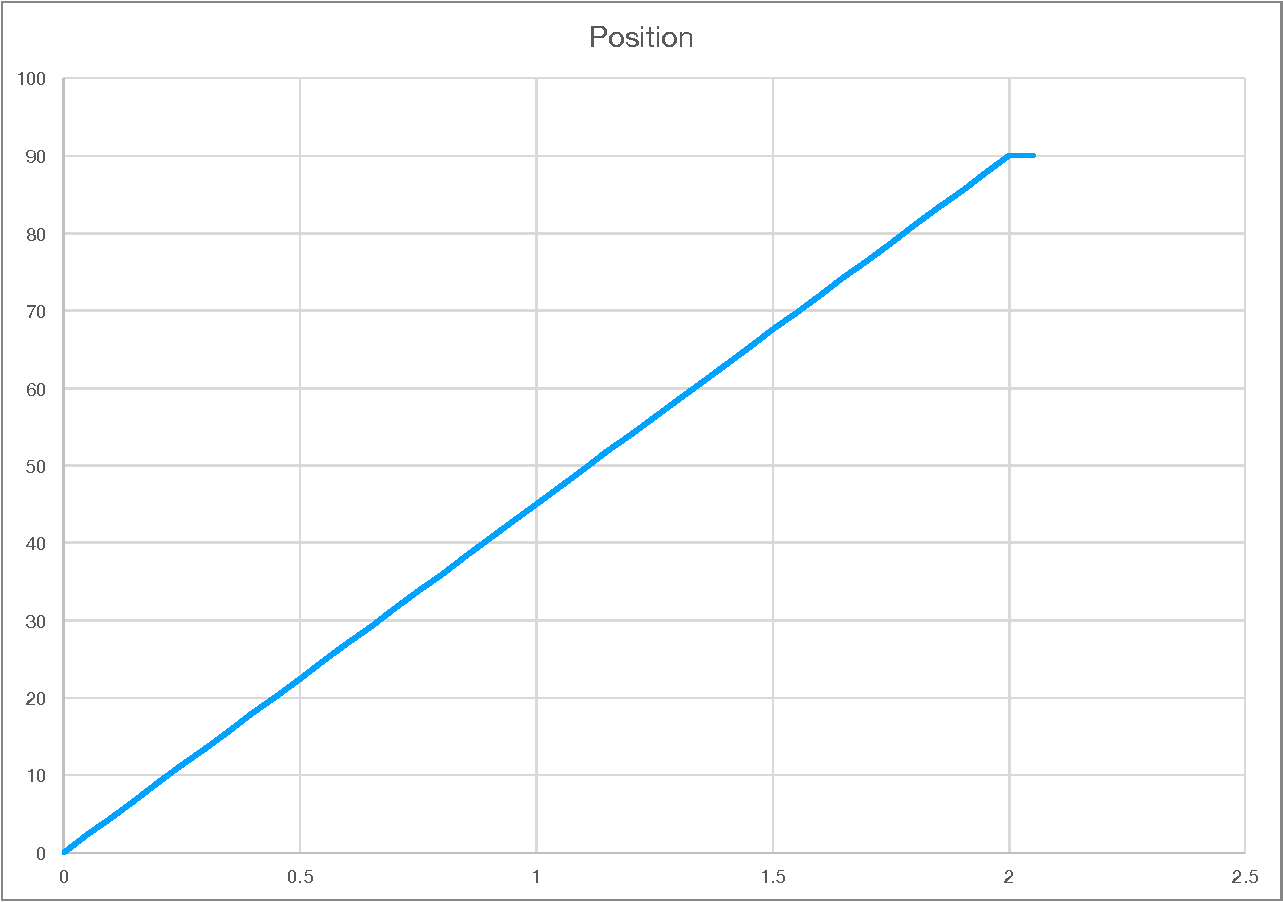
\includegraphics[width=0.7\textwidth]{position_simple.pdf}

Notice that the area under the velocity line is $2 \times 45$, the total
distance traveled. In fact, at any point in your drive, your distance
from the starting point is equal to the area under the velocity line.
% Diagram needed, explain why it is the area under the curve
% KA: https://www.khanacademy.org/math/ap-calculus-ab/ab-diff-contextual-applications-new/ab-4-2/e/interpret-motion-graphs

What if you:
\begin{itemize}
\item drive 50 km/hour for 45 minutes
\item rest for 15 minutes
\item continue driving 90 km/hour for 45 minutes
\item turn around and head back at 120 km/hour for 15 minutes
\end{itemize}
% KA: https://www.khanacademy.org/math/ap-calculus-ab/ab-diff-contextual-applications-new/ab-4-2/v/one-dimensional-motion-with-calculus

Now the graphs look a little more complex:

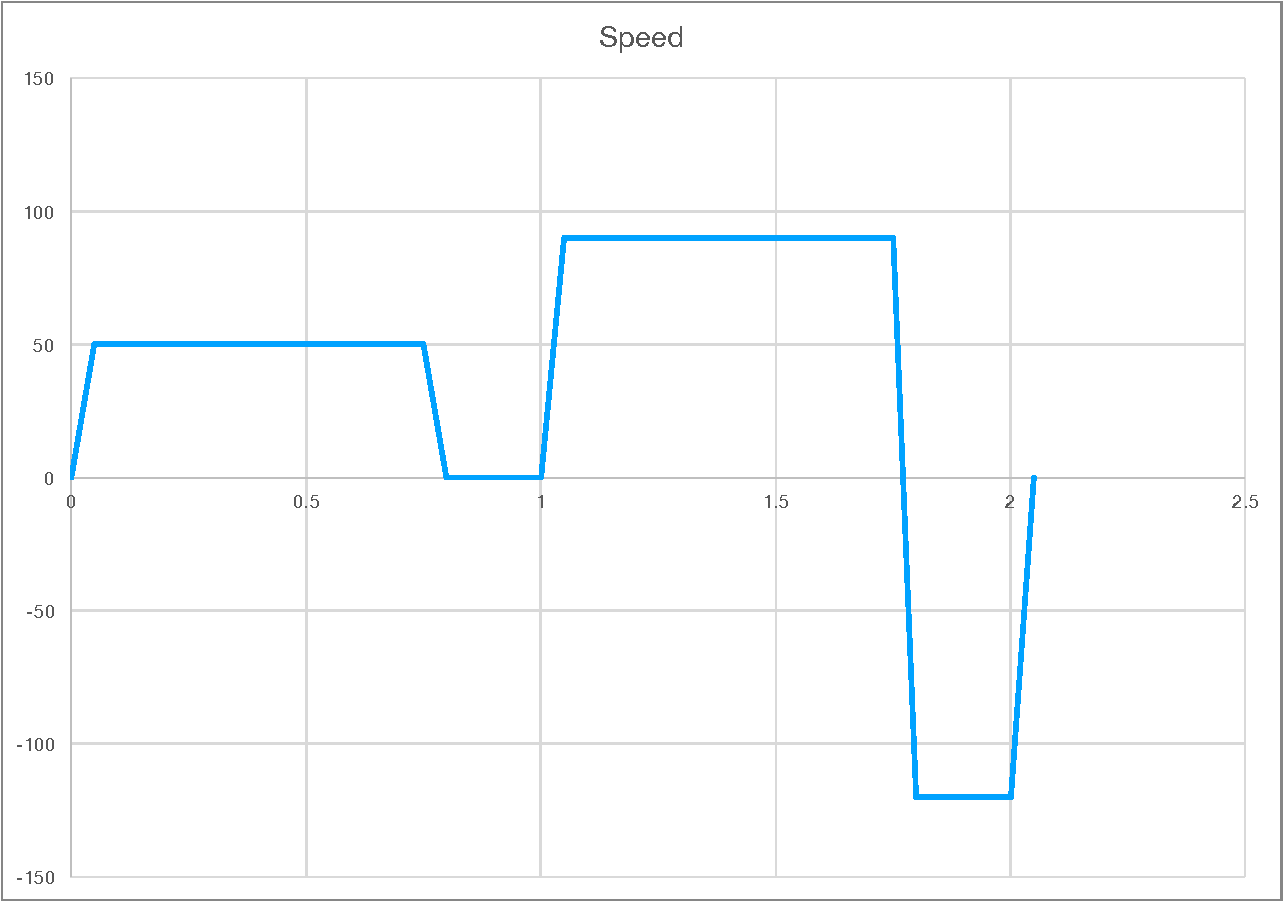
\includegraphics[width=0.7\textwidth]{speed_stops.pdf}

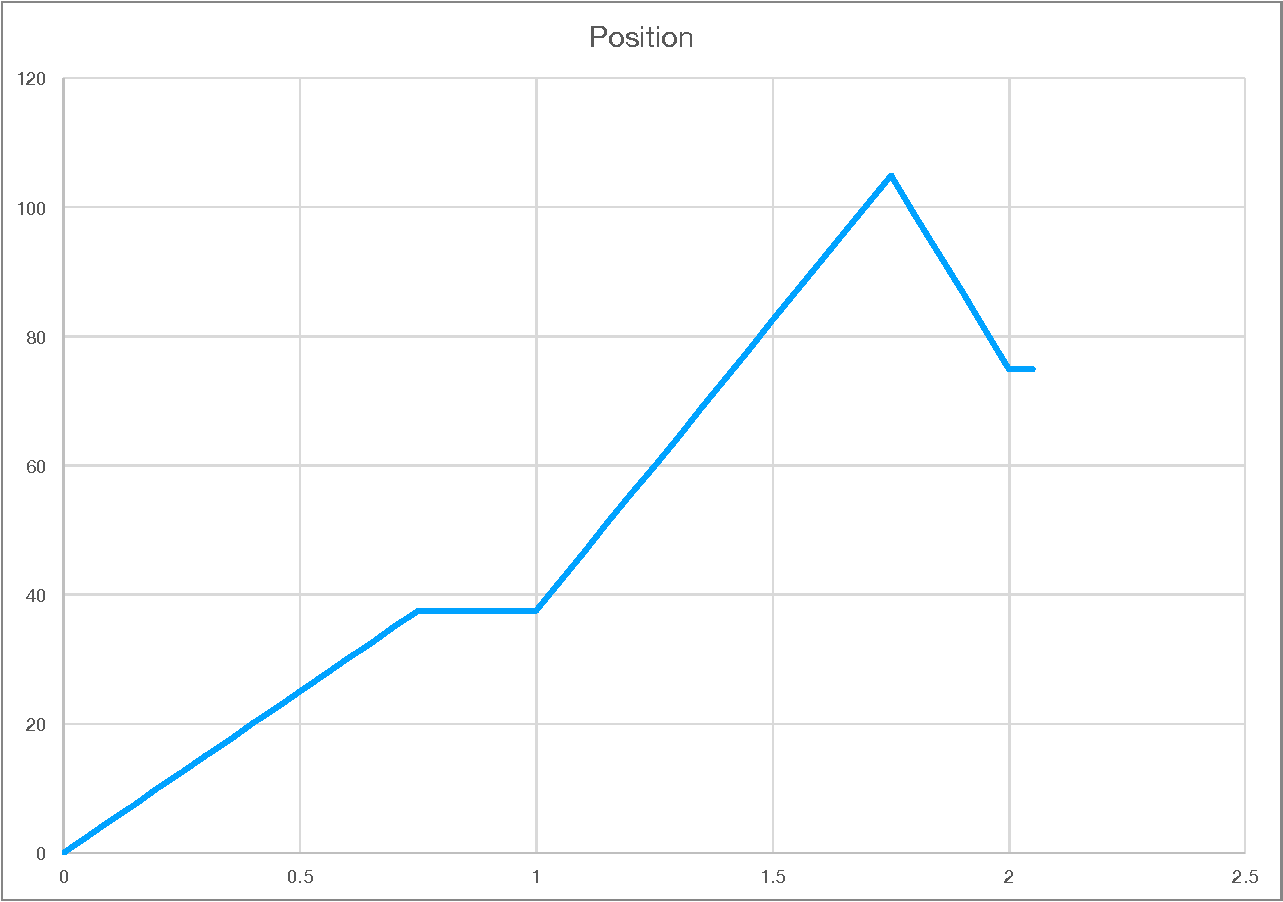
\includegraphics[width=0.7\textwidth]{position_stops.pdf}

It is still true that at any time, the position is equal to the
area under the graph up to that time. Notice that when the velocity goes
negative, it is subtracting from the position( negative velocity means going backwards).

Notice that when you are going faster, the slope of the position line
is steeper. When the slope of the position is negative, the velocity is
negative( the velocity is decreasing).

So we end up with two important ideas:
\begin{itemize}
\item If we plot the velocity, the position is equal to the area under the speed line.
\item If we plot the position, the velocity is equal to the slope of the position line.
\end{itemize}

\section{Acceleration}

Just as velocity represents the change in position over time,
acceleration represents the change in velocity over time.

What if, from a standstill, you accelerate smoothly 45 km/hour each
hour for one hour and 30 minutes. Then you stop accelerating for 15
minutes. Then you decelerate (or accelerate toward home) at a rate of
80 km/hour each hour for 15 minutes. Now we have three graphs: the
acceleration, the velocity, and the position

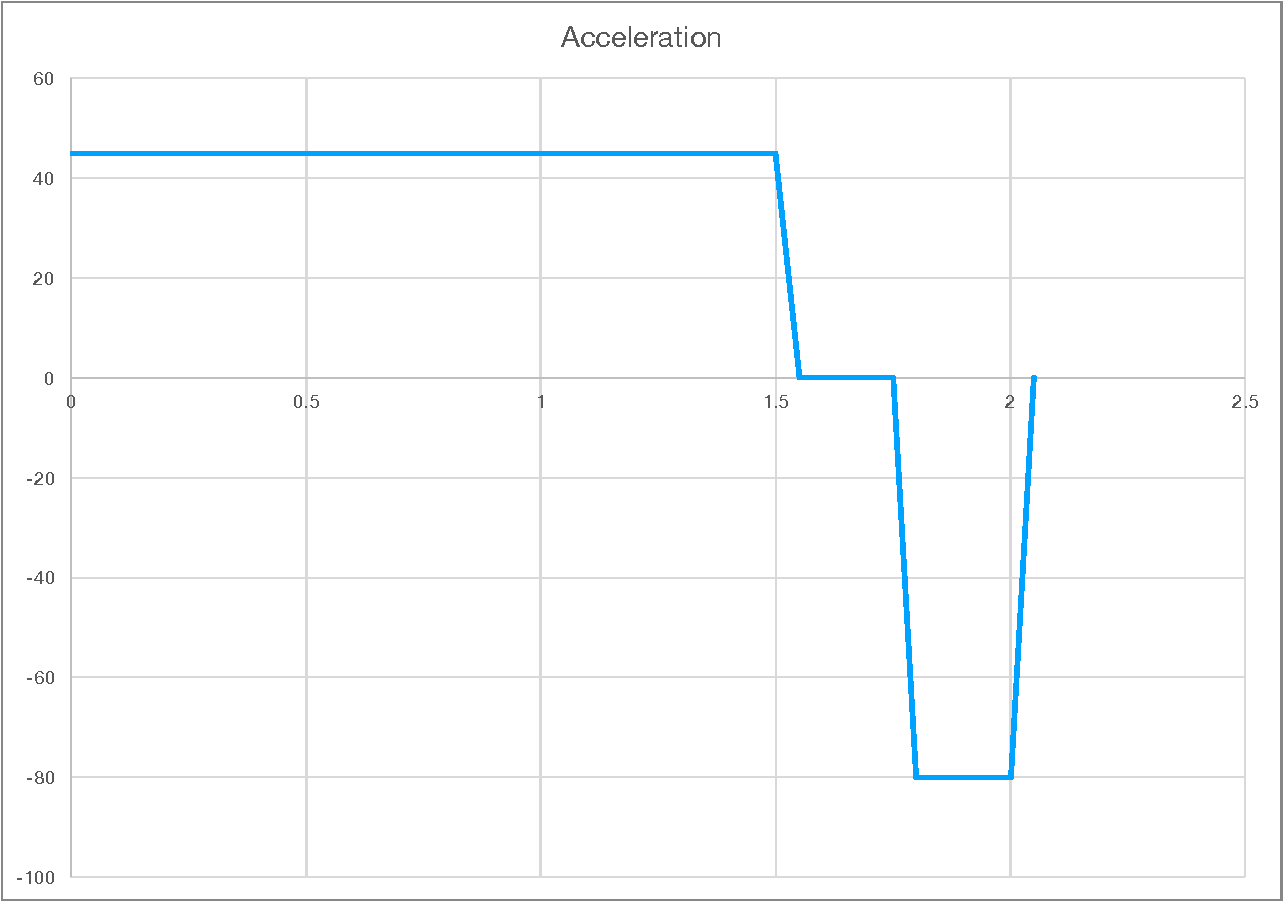
\includegraphics[width=0.7\textwidth]{acceleration_asp.pdf}

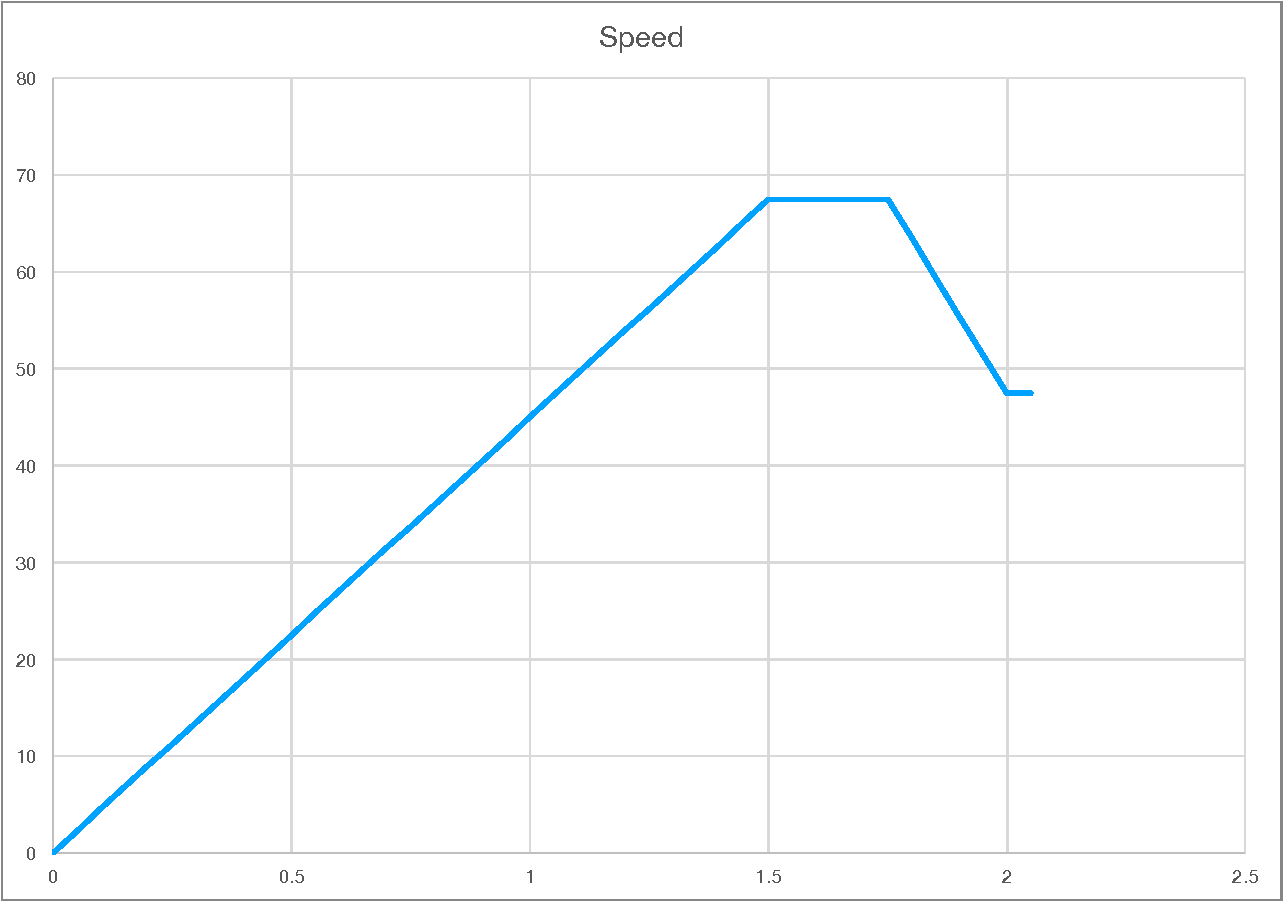
\includegraphics[width=0.7\textwidth]{speed_asp.pdf}

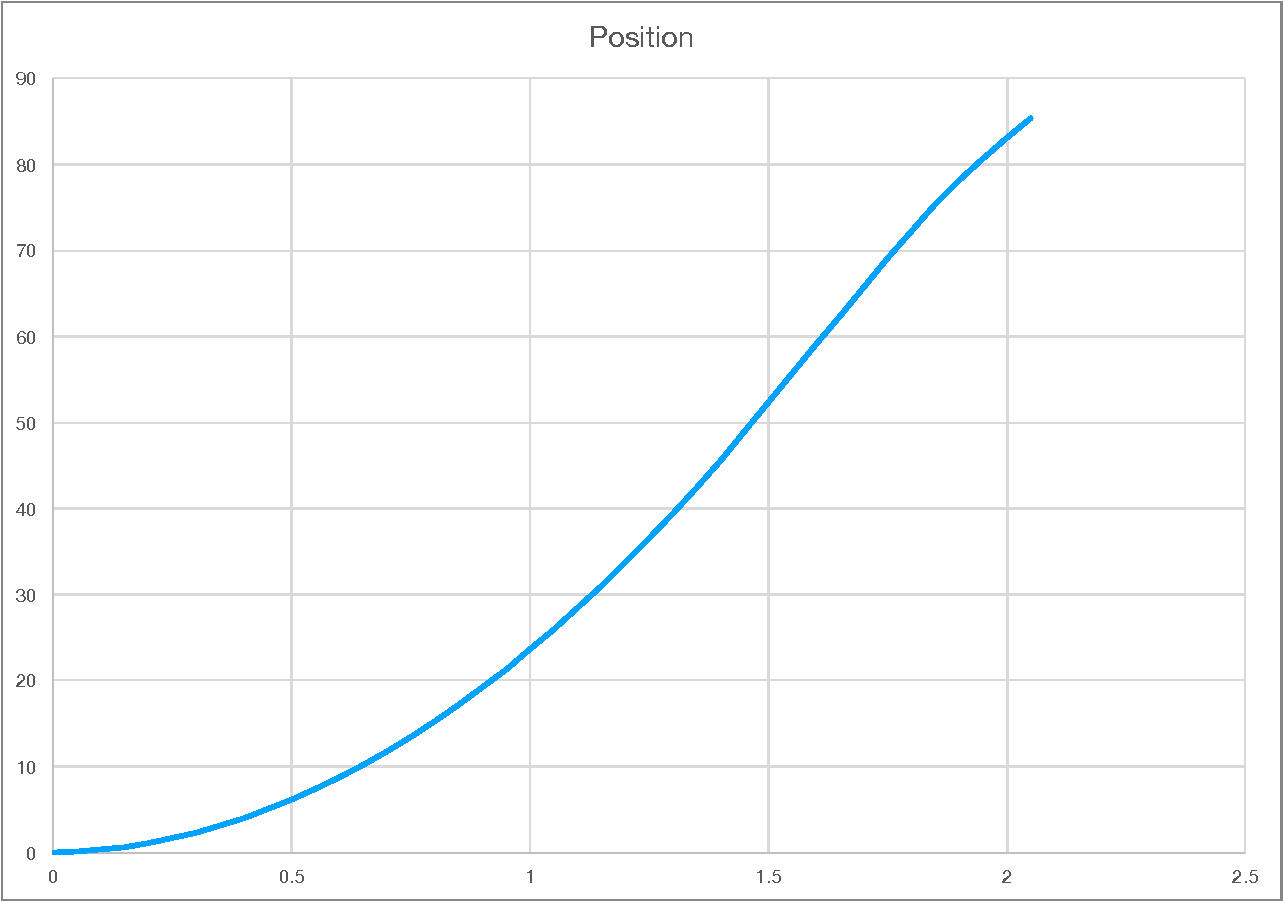
\includegraphics[width=0.7\textwidth]{position_asp.pdf}


So we end up with two important ideas:
\begin{itemize}
\item If we plot the acceleration, the velocity is equal to the area under the acceleration line.
\item If we plot the velocity, the acceleration is equal to the slope of the velocity line.
\end{itemize}

\section{Differentiation and Integration}

In calculus, we talk a lot about differentiation and integration.

\textit{Differentiation} is just finding the slope of a curve. If you give me
the position of an object over time, I will differentiate that to find
its velocity at any time. Once I have the velocity, I can differentiate
again to find its acceleration.

\textit{Integration} is just finding the area under a curve. If you give me
the initial speed of an object and its acceleration over time, I will
integrate that to find its velocity at any time. Then, if I know the
starting point of the object, I can integrate the velocity to find its
position at any time.

\section{Speed vs. Velocity, Distance vs. Position}

In casual conversation, we tend to use the words ``speed'' and
``velocity'' interchangeably. When we are solving problems, velocity
represents the change in position, and that can be pretty specific,
like ``It's velocity is 12 m/s due west.'' Velocity, then, can
have a direction and can be negative.

Speed, is just the magnitude of the velocity, like ``12 m/s''.  It is
a number that is never negative.
% ADD: Scalar vs Vector
% KA: https://www.khanacademy.org/math/ap-calculus-ab/ab-diff-contextual-applications-new/ab-4-2/v/one-dimensional-motion-with-calculus

Similarly, a position can be quite complex like ``12 km east of
Lexington.'' Distance is just a number, like ``12 km from Lexington.''
Distance is never negative.

% ADD: Distance vs Displacement
% KA: https://www.khanacademy.org/science/high-school-physics/one-dimensional-motion-2/distance-displacement-and-coordinate-systems-2/a/relative-motion-review-article

% ADD: Example interpreting all three graphs
% Video: https://www.google.com/url?sa=i&url=https%3A%2F%2Fwww.youtube.com%2Fwatch%3Fv%3DnUb7xfkc0Ac&psig=AOvVaw2cfsXUgDpoYlIRVKcfIMJP&ust=1653186487204000&source=images&cd=vfe&ved=0CAwQjRxqFwoTCPCdxtzF7_cCFQAAAAAdAAAAABAD
